\documentclass[12pt]{article}

\usepackage[T1]{fontenc}
\usepackage[margin=1in]{geometry}
\usepackage{amsmath,amssymb,amsthm,mathtools}
\usepackage{booktabs}
\usepackage{graphicx}
\usepackage{algorithm}
\usepackage[noend]{algpseudocode}
\usepackage{microtype}
\usepackage[numbers,sort&compress]{natbib}
\usepackage{xcolor}
\usepackage[colorlinks=true,linkcolor=blue!55!black,
  citecolor=blue!45!black,urlcolor=blue!55!black]{hyperref}

\theoremstyle{plain}
\newtheorem{theorem}{Theorem}
\newtheorem{proposition}[theorem]{Proposition}
\newtheorem{corollary}[theorem]{Corollary}
\newtheorem{lemma}[theorem]{Lemma}
\theoremstyle{definition}
\newtheorem{remark}[theorem]{Remark}

\newcommand{\reals}{\mathbf{R}}
\newcommand{\A}{\mathcal{A}}
\newcommand{\norm}[1]{\left\lVert #1\right\rVert}
\newcommand{\ip}[2]{\left\langle #1,#2\right\rangle}
\newcommand{\relu}[1]{\left(#1\right)_+}
\newcommand{\ones}{\mathbf{1}}
\newcommand{\diag}{\mathop{\bf diag}}
\newcommand{\Tr}{\mathop{\bf tr}}
\newcommand{\rank}{\mathop{\bf rank}}
\newcommand{\yhat}{\widehat y}
\DeclareMathOperator*{\argmax}{arg\,max}
\DeclareMathOperator*{\argmin}{arg\,min}

\title{Residual-Adaptive Column Generation for\\
Convex Two-Layer ReLU Fitting}
\author{Logan Bell}
\date{\today}

\begin{document}
\maketitle

\begin{center}
\small This work is licensed under a
\href{https://creativecommons.org/licenses/by/4.0/}{Creative Commons
Attribution 4.0 International License}.
\end{center}

\begin{abstract}
We consider fitting a scalar-output two-layer ReLU network with weight decay,
which is equivalent to a convex regularized fitting problem whose dictionary
contains one candidate feature for every direction on the unit sphere. The
convex problem is easy once the directions are fixed---it is an ordinary
lasso---but selecting the best missing direction is NP-hard. We propose
residual-adaptive column generation (RCG), which maintains a small working set
of directions, refits their coefficients, and searches for new directions
correlated with the current residual. When the restricted problems and the
search are solved exactly, the objective error after $t$ rounds is at most
$2\tau^2R^2/(t+4)$, where $\tau$ bounds the mass (coefficient sum) of an
optimum and $R$ bounds the atom norms; the bound carries no factor of the exponential number of
activation patterns, although the method need not terminate finitely.
Semidefinite relaxations give upper bounds on the search value, and hence dual
bounds, in exact arithmetic; our floating-point evaluation of these bounds is a
numerical estimate, not a certificate. In exploratory experiments the
implementation matches strong reference values on planted instances, maintains
its accuracy at a fixed working-set budget as random sampling degrades with
dimension,
and, on three real datasets against tuned Adam, AdamW, and SGD at budget-matched
wall clock, reaches an objective $45\%$ below the best tuned run on one dataset,
while on the other two the best tuned runs finish $3.4\%$ and $5.5\%$ lower;
these comparisons are exploratory, under budget-matched tuning grids. A
controlled benchmark of implementation choices identifies pricing search and
working-set consolidation as the dominant costs.
\end{abstract}

\section{Introduction}\label{s-intro}

Training a two-layer ReLU network is ordinarily a nonconvex problem, attacked
by stochastic local search over learning rates, initializations, and restarts.
For the scalar-output network with weight decay this is the problem
\begin{equation}\label{e-weight-decay}
\begin{array}{ll}
\mbox{minimize} & \displaystyle\frac12\norm{\sum_{j=1}^m\relu{Xw_j}b_j-y}_2^2
  +\frac\beta2\sum_{j=1}^m\left(\norm{w_j}_2^2+b_j^2\right),
\end{array}
\end{equation}
with variables the hidden weights $w_j\in\reals^d$ and output weights
$b_j\in\reals$; the data matrix $X\in\reals^{n\times d}$, responses
$y\in\reals^n$, width $m$, and decay parameter $\beta>0$ are given, and
$\relu{z}=\max(z,0)$ acts entrywise. A remarkable line of work
\citep{pilanci2020neural,ergen2021convex} showed that this nonconvex problem is
equivalent to a finite \emph{convex} program, so that global optimality---and
with it, an end to per-instance optimizer tuning---is at least meaningful.

The obstacle is size. The convex reformulation has one block of variables for
every \emph{activation pattern} the data admit, {\it i.e.}, every region of the
hyperplane arrangement $\{x_i^Tu=0\}$ cut by the rows of $X$
(Figure~\ref{f-chambers}). With $r=\rank X$, the number of such regions can
reach $2\sum_{k=0}^{r-1}\binom{n-1}{k}$, so the program cannot be written down
beyond small effective rank. Existing practice either samples a fixed random
subset of patterns and solves the restricted program
\citep{mishkin2022fast,kim2024sampling}, giving up any statement about the
patterns not sampled, or returns to nonconvex local search, giving up the
convex view entirely.

There is a third route. The convex program is an \emph{atomic-norm} problem
\citep{chandrasekaran2012convex}: its dictionary is the continuum of ReLU
features $\relu{Xu}$ with $\norm u_2\le1$, and one never needs the whole
dictionary, only a way to \emph{price} it---to find the feature most correlated
with a residual. Pricing over all exponentially many patterns collapses to a
single continuous problem in $u$ (Theorem~\ref{t-collapse}), so column
generation applies: keep a small working set of directions, solve the
restricted problem (an ordinary lasso), and add the direction most correlated
with the residual. We call this \emph{residual-adaptive column generation} (RCG):
every mechanism that grows or reshapes the working set is a function of the
current residual.

Convexity has moved the hard part into an oracle; it has not removed it.
Exact pricing is NP-hard (Theorem~\ref{t-hardness}). This paper takes that
oracle seriously in both directions. We prove exactly what an exact oracle
buys: full optimality conditions and an $O(1/t)$ rate with no factor of the
pattern count; we also prove that the method need not terminate finitely, even
in two dimensions. And we quantify what a cheap oracle costs: pricing is NP-hard and
APX-hard in general, polynomial at fixed effective rank, and admits computable
semidefinite upper bounds in exact arithmetic.

The practical solver is built to one invariant: heuristics may only propose,
and the objective disposes. Sketched multistart search, gated consolidation
(\S\ref{s-production}), and semidefinite rounding generate candidate directions, but
every acceptance is decided by the full-data objective of the original convex
problem, so approximation degrades only the quality of the search, never the
feasibility of the returned model or the objective being minimized. The
solver's gap diagnostics are numerical estimates, not certificates
(Remark~\ref{r-floating}).

\paragraph{This paper.}
Our principal contribution is the exact analysis of the ideal method and the
complexity landscape of its oracle: the pricing collapse and full
Karush--Kuhn--Tucker (KKT) conditions with active-atom saturation
(\S\ref{s-optimality}); the $2\tau^2R^2/(t+4)$ rate from an empty working set,
together with an explicit two-dimensional instance on which exact RCG runs
forever (\S\ref{s-ideal}); and the hardness of pricing on rational inputs,
already for the all-ones residual, complemented by fixed-rank tractability and
a sampling-coverage bound (\S\ref{s-pricing}). A supporting contribution is a
low-rank semidefinite dual (\S\ref{s-small-cone})---a $d\times d$ program
rather than $n\times n$---that upper-bounds the price in exact arithmetic and turns any valid bound
into a dual lower bound on the fitting problem (\S\ref{s-bounds}). The
empirical contribution is an objective-preserving solver
(\S\ref{s-production}) and two grades of evidence for it
(\S\ref{s-experiments}): exploratory comparisons on planted and real data
against tuned first-order baselines and random pattern sampling, and a
controlled, preregistered benchmark of implementation choices with independent
objective replay. Several individual results adapt known arguments, and we
credit them where they appear; the hardness reduction, the nontermination
construction, the small-cone identity, and the failure example for mixed-sign
rounding are, to our knowledge, new.

\subsection{Prior work}\label{s-prior}

\paragraph{Convex ReLU formulations.}
\citet{pilanci2020neural} derive the finite convex reformulation of
weight-decay training by enumerating activation patterns; \citet{ergen2021convex}
extend the equivalence, and the connection between weight decay and
$\ell_1$-type regularization of the network's function goes back at least to
\citet{neyshabur2015search,savarese2019infinite}. The equivalence we state in
\S\ref{s-objective} is a width-qualified version of these results. Our
departure is to keep the dictionary continuous and search it, rather than
enumerate or sample it.

\paragraph{Continuous dictionaries and conditional gradient.}
Incremental atom insertion for convex neural networks originates with
\citet{bengio2006convex} and is developed for general continuous dictionaries
by \citet{bach2017breaking}; the algorithmic template is Frank--Wolfe
\citep{frank1956algorithm,jaggi2013revisiting,clarkson2010coresets,
lacostejulien2015global}, and alternating-descent conditional gradient adds
local motion of active atoms \citep{boyd2017adcg,eftekhari2019equivalence}.
Our rate theorem is the penalized fully-corrective rate of this literature,
proved directly for the signed-atomic objective, with antecedents in greedy
approximation \citep{barron1993universal,clarkson2010coresets}; the
nontermination example appears to be new and is specific to the continuous
ReLU dictionary.

\paragraph{Selected-pattern solvers.}
SCNN \citep{mishkin2022fast} and CRONOS \citep{feng2024cronos} solve the
convex program restricted to a sampled or selected set of patterns, with
accelerated first-order, augmented-Lagrangian, and GPU-oriented methods;
\citet{kim2024sampling} analyze what random sampling achieves. These are
strong solvers of the restricted problem. Their residuals do not test the
patterns they omit, which is precisely the separation step
(\S\ref{s-optimality}) this paper studies; the random-pattern baseline in
\S\ref{s-exp-curse} isolates that difference while holding the rest of the
method fixed.

\paragraph{Hardness.}
Training-time hardness for depth-2 ReLU networks is established by
\citet{goel2021tight} and refined by parameterized results
\citep{froese2022computational}; \citet{bach2017breaking} already notes the
hardness of the incremental (oracle) step for related dictionaries, and
\citet{boob2022complexity} prove hardness of fitting a single ReLU, the
problem closest to the pricing functional itself.
Theorem~\ref{t-hardness} localizes hardness in the pricing functional itself,
on rational inputs, already at the all-ones residual, and adds APX-hardness
with a no-PTAS consequence via a rational Max-Cut reduction.

\paragraph{Semidefinite bounds.}
Our price bounds use the positive-semidefinite Boolean quadratic machinery of
\citet{nesterov1998semidefinite} and \citet{goemans1995improved}. The diagonal
dual we start from is classical---it is the Delorme--Poljak bound for Max-Cut
\citep{delorme1993laplacian}---and our contribution is the closed
\emph{small-cone} form, a $d\times d$ dual with an explicit recovery map that
tolerates inexact inner solutions in exact arithmetic.

\paragraph{Outline.}
\S\ref{s-objective} sets up the three equivalent problems.
\S\ref{s-optimality} develops pricing, the optimality conditions, and the dual.
\S\ref{s-ideal} analyzes ideal exact RCG. \S\ref{s-pricing} maps the
complexity of pricing, and \S\ref{s-bounds} constructs computable price
bounds. \S\ref{s-production} describes the solver, and \S\ref{s-experiments}
reports the numerical evidence. \S\ref{s-conclusion} concludes.

\section{The convex fitting problem}\label{s-objective}

Throughout, $X\in\reals^{n\times d}$ has rows $x_1^T,\ldots,x_n^T$, the
responses are $y\in\reals^n$, and $r=\rank X$ is the effective rank. For a
direction $u\in\reals^d$ with $\norm u_2\le1$, the \emph{ReLU atom} $a(u)=
\relu{Xu}\in\reals^n$ is the feature vector the hidden neuron $u$ contributes
on the data. Define the compact signed atom set
\[
  \A=\{\,\sigma\relu{Xu}\ : \ \norm u_2\le1,\ \sigma\in\{-1,1\}\,\}
  \subset\reals^n .
\]

The finite-atom fitting problem is
\begin{equation}\label{e-finite-atom}
\begin{array}{ll}
\mbox{minimize} & \displaystyle
  F(\alpha,U)=\frac12\norm{\sum_{j=1}^P\alpha_j\relu{Xu_j}-y}_2^2
  +\lambda\sum_{j=1}^P|\alpha_j|,
\end{array}
\end{equation}
with variables the number of atoms $P$ (a nonnegative integer), the signed
coefficients $\alpha\in\reals^P$, and the directions $u_j$ with
$\norm{u_j}_2\le1$; the data $X$, $y$, and the penalty $\lambda>0$ are given.
The direction parameterization makes \eqref{e-finite-atom} nonconvex as
written, but it is a finite representation of a convex problem. Let
$\gamma_{\A}$ be the atomic gauge of $\A$,
\[
  \gamma_{\A}(\yhat)
  =\inf\Big\{\sum_jc_j \ \Big|\ \yhat=\sum_jc_ja_j,\ c_j\ge0,\ a_j\in\A\Big\},
\]
with value $+\infty$ outside the span of $\A$. We call $\sum_j c_j$ the
\emph{mass} of the representation. The convex problem is
\begin{equation}\label{e-atomic}
\begin{array}{ll}
\mbox{minimize} & \frac12\norm{\yhat-y}_2^2+\lambda\,\gamma_{\A}(\yhat),
\end{array}
\end{equation}
with variable the prediction $\yhat\in\reals^n$. Since $\A$ is compact and
contains $0$, its convex hull is compact, the gauge is closed, and the infimum
in $\gamma_{\A}$ is attained; allowing arbitrary finite representations in
\eqref{e-finite-atom} therefore gives exactly the optimal value of
\eqref{e-atomic}.

The weight-decay problem \eqref{e-weight-decay} is the same problem again,
provided the network is wide enough.

\begin{proposition}[Width-qualified equivalence]\label{p-equivalence}
Let $\lambda=\beta>0$, and let $m^\star$ be the least number of signed atoms in
a minimum-mass representation of some optimum of~\eqref{e-atomic}. If $m\ge
m^\star$, then problems \eqref{e-weight-decay}, \eqref{e-finite-atom}, and
\eqref{e-atomic} have the same optimal value; every optimal atomic
representation with at most $m$ atoms yields an optimal network by the
construction in the proof, and every optimal network yields an optimal atomic
representation by normalization.
\end{proposition}

\begin{proof}
For a nonzero neuron, put $u=w/\norm w_2$ and $\alpha=b\norm w_2$. Positive
homogeneity of the ReLU preserves the neuron's prediction, while
\[
  \frac\beta2\left(\norm w_2^2+b^2\right)\ \ge\ \beta\,|b|\,\norm w_2
  \ =\ \lambda|\alpha|,
\]
with equality when the two layers are balanced, $\norm w_2=|b|$. Conversely,
an atom with coefficient $\alpha$ is realized by the balanced neuron
$w=\sqrt{|\alpha|}\,u$, $b=\mathop{\bf sign}(\alpha)\sqrt{|\alpha|}$, and the
width hypothesis permits this construction atom by atom for an optimal
representation.
\end{proof}

Corollary~\ref{c-width} below shows $m\ge n$ is always sufficient. We do not
claim the equivalence for an arbitrary smaller width.

\begin{figure}[tb]
  \centering
  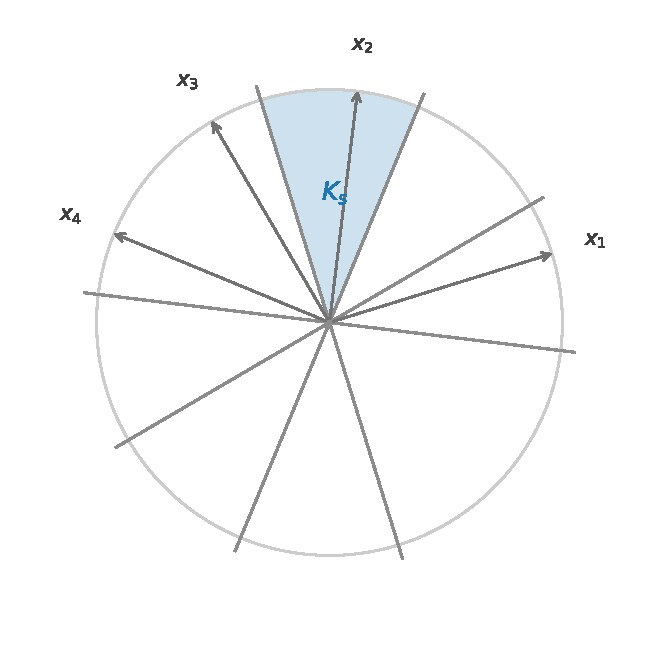
\includegraphics[width=0.5\linewidth]{figures/chamber_arrangement.pdf}
  \caption{A central arrangement in $\reals^2$ with $n=4$ data rows. Each row
  $x_i$ contributes the hyperplane $x_i^Tu=0$; the full-dimensional regions
  are the chambers, and the shaded cone is the chamber $K_s$ on which all four
  rows are active, $s=(1,1,1,1)$. Every ReLU atom is linear on each chamber.}
  \label{f-chambers}
\end{figure}

\paragraph{Chambers.}
The finite convex program of \citet{pilanci2020neural} is a third
representation of the same gauge, and it supplies the geometry we use
throughout. Work in the row span of $X$, of dimension $r$. A \emph{chamber} is
a full-dimensional region of the central arrangement $\{x_i^Tu=0 :
\norm{x_i}_2>0\}$ restricted to the row span (the arrangement is
\emph{essential} there: the nonzero rows span it). For a binary gate vector
$s\in\{0,1\}^n$ write $D_s=\diag(s)$, where $\diag(v)$ is the diagonal matrix
with diagonal $v$, and define the closed cone
\[
  K_s=\{u\in\reals^d \mid (2D_s-I)Xu\ge0\},
\]
the set of directions whose sign pattern is consistent with $s$. The cone
$K_s$ lives in $\reals^d$ and contains the null space of $X$; its intersection
with the row span is the corresponding chamber closure. Let $\mathcal S$ be
the set of gate vectors of full-dimensional chambers. For $u\in K_s$ we have
$D_sXu=\relu{Xu}$, including on the boundary, and the chamber program is
\begin{equation}\label{e-chamber}
\begin{array}{ll}
\mbox{minimize} & \displaystyle
 \frac12\norm{\sum_{s\in\mathcal S}D_sX(v_s-w_s)-y}_2^2
 +\lambda\sum_{s\in\mathcal S}\left(\norm{v_s}_2+\norm{w_s}_2\right),
\end{array}
\end{equation}
with variables the chamber blocks $v_s,w_s\in K_s$. Normalizing a nonzero
block, $v_s=\norm{v_s}_2u$ with $u\in K_s$, produces the signed atom
$\norm{v_s}_2\relu{Xu}$, so every feasible point of \eqref{e-chamber} is a
representation in \eqref{e-atomic} of no larger cost; conversely, grouping the
atoms of a representation by chamber and sign and using the triangle
inequality on each group's directions (each $K_s$ is convex) gives a chamber
point of no larger cost. The two problems have the same value. Note one consequence: the restricted problem over any finite set
of atoms needs \emph{no} cone constraints---each ReLU atom is a valid feature
of its own chamber automatically---so the restricted problem is an ordinary
lasso.

\begin{proposition}[Chamber count]\label{p-chamber-count}
If $r\ge1$, the number of full-dimensional chambers is at most
\[
  2\sum_{k=0}^{r-1}\binom{n-1}{k},
\]
with equality when all $n$ rows are nonzero and in general position in the
row span (every subset of at most $r$ of them linearly independent). If $r=0$ there is
one zero-dimensional chamber closure.
\end{proposition}

\begin{proof}
The bound is the classical central-arrangement count
\citep[Theorem~2]{cover1965geometrical}; see also
\citet[Chapter~2]{stanley2007arrangements}. Repeated or dependent rows can
make it strict.
\end{proof}

Sign patterns $\ones\{Xu\ge0\}$ attained only on arrangement boundaries need
not correspond to full-dimensional chambers, but chamber closures suffice for
every ReLU atom: every point of the row span lies in the closure of some
full-dimensional region, and a row whose sign changes among the incident
regions satisfies $x_i^Tu=0$, leaving the gated feature unchanged.

\section{Pricing and exact optimality}\label{s-optimality}

The chamber count of Proposition~\ref{p-chamber-count} is the size obstacle.
This section shows that testing optimality does not require touching it: the
exponential family of chamber tests collapses to one continuous problem, and
together with a saturation condition on the active atoms it characterizes
global optimality exactly.

For a residual $\nu\in\reals^n$, define the \emph{price} of a direction set:
the chamber-restricted price and the global price are
\[
  \rho_s(\nu)=\max_{u\in K_s,\ \norm u_2\le1}\nu^TD_sXu,
  \qquad
  \rho(\nu)=\max_{\norm u_2\le1}\nu^T\relu{Xu}.
\]
The support function of the signed atom set is
$p(\nu)=\max\{\rho(\nu),\rho(-\nu)\}$, the \emph{signed price}. Dual
feasibility of $\nu$ is the family of \emph{polar inequalities} $\nu^Ta\le
\lambda$ for all $a\in\A$, equivalently $p(\nu)\le\lambda$. In
column-generation language, an atom with $\nu^Ta>\lambda$ is a
\emph{violator}, and finding one is \emph{separation}.

\begin{theorem}[Pricing collapse]\label{t-collapse}
For every $\nu\in\reals^n$,
\[
  \max_{s\in\mathcal S}\rho_s(\nu)=\rho(\nu).
\]
\end{theorem}

\begin{proof}
For $u\in K_s$ with $\norm u_2\le1$ we have $D_sXu=\relu{Xu}$, so each
chamber-restricted value is at most $\rho(\nu)$. Conversely every unit
direction lies in the closure of an incident full-dimensional chamber and
attains the same ReLU feature there.
\end{proof}

So the continuum of directions prices exactly as the finitely many chambers
do; the difficulty is not the continuum, and separation needs no enumeration.

Dual feasibility alone, however, does not certify an arbitrary feasible
representation. Take $X=[1]$, $y=2$, $\lambda=1/2$, and represent the
prediction $\yhat=2$ by coefficient $2$ on the atom $\relu{X\cdot1}=1$, so the
mass is $\ell=2$ and the cost is $0+\lambda\cdot2=1$. The residual is zero,
hence both prices are zero and dual feasibility holds---yet the optimum
$\yhat=3/2$ has cost $7/8$. What is missing is that each \emph{active} atom
must saturate its polar inequality.

For a representation $\yhat=\sum_jc_ja_j$ with $c_j\ge0$ and $a_j\in\A$, write
$\ell=\sum_jc_j$ for its mass and
$J(\yhat,\ell)=\tfrac12\norm{\yhat-y}_2^2+\lambda\ell$ for its cost; for the
corresponding $(\alpha,U)$ this equals $F(\alpha,U)$ in
\eqref{e-finite-atom}.

\begin{theorem}[Full KKT conditions]\label{t-kkt}
Let $\yhat=\sum_jc_ja_j$ with $c_j\ge0$ and $a_j\in\A$, and put
$\ell=\sum_jc_j$ and $\nu=y-\yhat$. This representation attains the optimal
value of~\eqref{e-atomic} (equivalently, $\yhat$ is optimal and
$\ell=\gamma_{\A}(\yhat)$) if and only if
\begin{equation}\label{e-kkt}
  p(\nu)\le\lambda
  \qquad\text{and}\qquad
  \nu^Ta_j=\lambda\ \ \text{for every }c_j>0 .
\end{equation}
Equivalently, in the chamber program \eqref{e-chamber}, both one-sided prices
$\rho(\pm\nu)$ are at most $\lambda$ and every nonzero block saturates its polar inequality.
Every active normalized block is therefore a global price maximizer at value
$\lambda$; an inactive chamber may also contain a maximizer.
\end{theorem}

\begin{proof}
Assume \eqref{e-kkt}. For any competing representation $(\yhat',\ell')$, dual
feasibility gives $\nu^T\yhat'\le\lambda\ell'$, while active saturation gives
$\nu^T\yhat=\lambda\ell$. Hence
\[
 J(\yhat',\ell')-J(\yhat,\ell)
 =\frac12\norm{\yhat'-\yhat}_2^2-\nu^T(\yhat'-\yhat)+\lambda(\ell'-\ell)
 \ge\frac12\norm{\yhat'-\yhat}_2^2 .
\]
Conversely, at a representation attaining the optimal value, adding a small
amount of any signed atom shows $\nu^Ta\le\lambda$, and a two-sided scalar
variation of each positive coefficient forces equality. In the chamber
program, pairing each nonzero block's KKT inclusion with the block itself
gives the same saturation condition, because the normal-cone term is
orthogonal to the block.
\end{proof}

\begin{corollary}[Exact restricted stopping]\label{c-restricted-stop}
Let a representation be an exact minimizer of the restricted problem over a
finite atom set. Then its active saturation conditions already hold, and the
representation is globally optimal for \eqref{e-atomic} if and only if exact
pricing of both signs gives $\rho(\nu)\le\lambda$ and $\rho(-\nu)\le\lambda$.
\end{corollary}

\begin{proof}
Apply Theorem~\ref{t-kkt} to the finite dictionary of the restricted problem:
exact restricted optimality yields saturation of its active atoms. Global
optimality then reduces to the two remaining price inequalities.
\end{proof}

The corollary concerns an exact restricted minimizer. It does not apply after
an unresolved approximate solve, and this is exactly the premise the practical
solver of \S\ref{s-production} gives up.

\begin{proposition}[Sparse optimal representation]\label{p-sparse}
Problem~\eqref{e-atomic} admits an optimum represented by at most $n$ signed
atoms, hence by at most $n$ chamber blocks.
\end{proposition}

\begin{proof}
Choose a finite minimum-mass representation of an optimal prediction (finite
existence follows from Carath\'eodory's theorem applied in $\reals^n$). If
more than $n$ coefficients are positive, there is a nonzero $h$ with
$\sum_jh_ja_j=0$. Active saturation in Theorem~\ref{t-kkt} gives
$\lambda\sum_jh_j=\nu^T\sum_jh_ja_j=0$, so moving the coefficients along $h$
until one hits zero preserves both the prediction and the mass. Repeat.
\end{proof}

The same argument applies verbatim to any finite restricted problem. The
result is existential: it bounds neither every optimum nor the working set of
an algorithm.

\begin{corollary}\label{c-width}
In Proposition~\ref{p-equivalence}, width $m\ge n$ is always sufficient.
\end{corollary}

\paragraph{The dual.}
The dual of problem \eqref{e-atomic} will let us convert price bounds into
objective bounds. It is
\begin{equation}\label{e-dual}
\begin{array}{ll}
\mbox{maximize} & D(\xi)=\xi^Ty-\frac12\norm\xi_2^2\\
\mbox{subject to} & p(\xi)\le\lambda,
\end{array}
\end{equation}
with variable $\xi\in\reals^n$; the constraint is the pair of polar
constraints $\rho(\pm\xi)\le\lambda$. Weak duality is immediate: for any
representation $(\yhat,\ell)$ and any feasible $\xi$,
\[
  J(\yhat,\ell)\ \ge\ \frac12\norm{\yhat-y}_2^2+\xi^T\yhat
  \ =\ D(\xi)+\frac12\norm{\yhat-y+\xi}_2^2\ \ge\ D(\xi),
\]
where the first inequality uses $\lambda\ell\ge\sum_jc_j\,\xi^Ta_j
=\xi^T\yhat$. A feasible $\xi$ therefore certifies
$J^\star\ge D(\xi)$, where $J^\star$ denotes the optimal value. Restricting the polar constraints to a finite working set gives the
restricted dual, and since maximizing $D$ is minimizing
$\norm{\xi-y}_2^2/2$, the exact restricted dual solution is the Euclidean
projection of $y$ onto the restricted constraint set. This projection
characterization drives the construction in
Appendix~\ref{a-nontermination}.

\section{Ideal exact column generation}\label{s-ideal}

Corollary~\ref{c-restricted-stop} suggests the method: solve the restricted
problem, price the residual, add the violator, repeat. We first analyze the
ideal version, in which every step is exact; Algorithm~\ref{alg-ideal} states
one \emph{canonical round}. The restricted problem over the working set is
called the \emph{restricted master}, following column-generation usage; as
noted in \S\ref{s-objective} it is an ordinary lasso, and the \emph{empty
master} (empty working set) has cost $J(0,0)$. A signed atom is
$\sigma\relu{Xu}$, so a working set of signed atoms and a working set of
signed directions are the same object, and we use whichever is convenient.

\begin{algorithm}[tb]
\caption{Ideal exact RCG (one canonical round)}\label{alg-ideal}
\begin{algorithmic}[1]
\Require data $X,y$; penalty $\lambda$; working set $W$ of signed atoms
\State \textbf{master:} solve the restricted master over $W$ exactly,
  obtaining the prediction $\yhat_t$, mass $\ell_t$, and residual
  $\nu_t=y-\yhat_t$
\State \textbf{price:} compute $p_t=p(\nu_t)$ and an attaining signed atom
  $a_t$ exactly
\State \textbf{stop} if $p_t\le\lambda$: the iterate is globally optimal
  (Corollary~\ref{c-restricted-stop})
\State \textbf{add:} $W\gets W\cup\{a_t\}$, retaining the current
  representation
\end{algorithmic}
\end{algorithm}

This is fully corrective column generation---all retained coefficients are
refit every round---in the standard exchange template for a continuous
dictionary \citep{bach2017breaking,jaggi2013revisiting}. Let $J_t$ be the
restricted-master cost after $t$ canonical rounds, with $J_0=J(0,0)$.

\begin{theorem}[Exact canonical-round rate]\label{t-rate}
Suppose an optimum of \eqref{e-atomic} has a representation of mass at most
$\tau$, and let
\[
  R=\max_{a\in\A}\norm a_2\le\sigma_{\max}(X).
\]
Starting from the empty master, canonical exact rounds satisfy
\begin{equation}\label{e-rate}
  J_t-J^\star\le\frac{2\tau^2R^2}{t+4}.
\end{equation}
If $\tau R=0$, the empty master is already optimal.
\end{theorem}

\begin{proof}
Let $\Delta_t=J_t-J^\star$. Exact restricted-master optimality gives the
saturation identity $\nu_t^T\yhat_t=\lambda\ell_t$
(Corollary~\ref{c-restricted-stop}). Let an optimal representation
$(\yhat^\star,\ell^\star)$ have mass $\ell^\star\le\tau$. Convexity of the
squared loss gives
\begin{equation}\label{e-price-gap}
  \Delta_t
  \le\nu_t^T(\yhat^\star-\yhat_t)+\lambda(\ell_t-\ell^\star)
  =\nu_t^T\yhat^\star-\lambda\ell^\star
  \le(p_t-\lambda)\,\ell^\star .
\end{equation}
In particular, if $\Delta_t>0$ then $p_t>\lambda$ and
$\Delta_t\le\tau(p_t-\lambda)$. Keeping the current coefficients and adding
the priced atom with the scalar step
\[
  \delta=\frac{p_t-\lambda}{\norm{a_t}_2^2}
\]
decreases the cost by exactly $(p_t-\lambda)^2/(2\norm{a_t}_2^2)$; we call
this update the \emph{one-coordinate comparator}. Exact reoptimization can
only do better, so
\[
  \Delta_{t+1}\le\Delta_t-\frac{\Delta_t^2}{2\tau^2R^2}.
\]
Write $C=2\tau^2R^2$. Full KKT at an optimum gives
$\Delta_0=J(0,0)-J^\star\le\norm{\yhat^\star}_2^2/2\le C/4$, which matches
\eqref{e-rate} at $t=0$; and if $\Delta_t\le C/(t+4)$ then
$\Delta_{t+1}\le C(t+3)/(t+4)^2\le C/(t+5)$.
\end{proof}

The bound involves no chamber count and no dimension; the data enter only
through $\tau$, the mass of an optimum, and $R$, the largest atom norm.
Compare Proposition~\ref{p-chamber-count}: enumeration-based formulations
carry the chamber count in their problem size, whereas the rate
\eqref{e-rate} does not. Column generation pays for the dictionary through the pricing oracle
instead, which motivates the study of pricing complexity in
\S\ref{s-pricing}.

Practical solvers do more between rounds than add one atom: they re-aim
directions, merge atoms, prune, and cap. The rate survives such moves under
explicit conditions.

\begin{proposition}[Optional moves preserve the rate conditionally]
\label{p-optional}
Consider a counted round (one that advances the index $t$ in
Theorem~\ref{t-rate}) that begins at an exact KKT point of the represented
finite master and interposes arbitrary modifications of the working set and
representation. The recurrence of Theorem~\ref{t-rate} holds for the round if:
(i) exact signed pricing is evaluated at that KKT point and returns an exact
maximizer $a_t$; (ii) the represented atoms and $a_t$ are all columns of the
next master, so the one-coordinate comparator remains feasible; (iii) any
replacement of the representation has exact cost no larger than the
comparator's; and (iv) the next counted round again begins with an exact
master solve.
\end{proposition}

\begin{proof}
Conditions (i)--(ii) reproduce the inequality \eqref{e-price-gap} and keep the
comparator available to the next exact solve; (iii) can only improve on the
comparator's decrease; (iv) restores the saturation identity used at the start
of the next round.
\end{proof}

The conditions are not vacuous: chamber compression (\S\ref{s-production}) is
an exact, cost-nonincreasing replacement satisfying (ii) and (iii); the
production solver nevertheless forfeits (i) and (iv) through its numerical
master.

Even with everything exact, the method need not stop.

\begin{theorem}[No finite termination]\label{t-nontermination}
There is an instance with $n=d=2$ on which exact RCG, started from a
two-atom master, adds a new atom in every round: no finite round passes the
price test, although $J_t\to J^\star$. Concretely, $X=I_2$, $\lambda=1$, and
$y=4u_{\pi/3}$, where $u_\theta=(\cos\theta,\sin\theta)$, initialized with
$u_0$ and $u_{\pi/2}$.
\end{theorem}

On this instance the exact restricted dual is a Euclidean projection of $y$
onto the accumulated polar constraints, and exact pricing adds the angular
midpoint of the two constraints bracketing $\pi/3$ (Figure~\ref{f-bisection});
since $\pi/3$ is never a dyadic midpoint of $[0,\pi/2]$, every round finds a
strict violator. Appendix~\ref{a-nontermination} gives the proof.
Proposition~\ref{p-sparse} is not contradicted: the full problem admits a
sparse optimal representation, while the accumulated dictionary keeps growing.
Tolerance-based stopping is therefore not an implementation shortcut: by
Theorem~\ref{t-nontermination}, even the ideal method cannot rely on exact
termination.

\begin{figure}[tb]
  \centering
  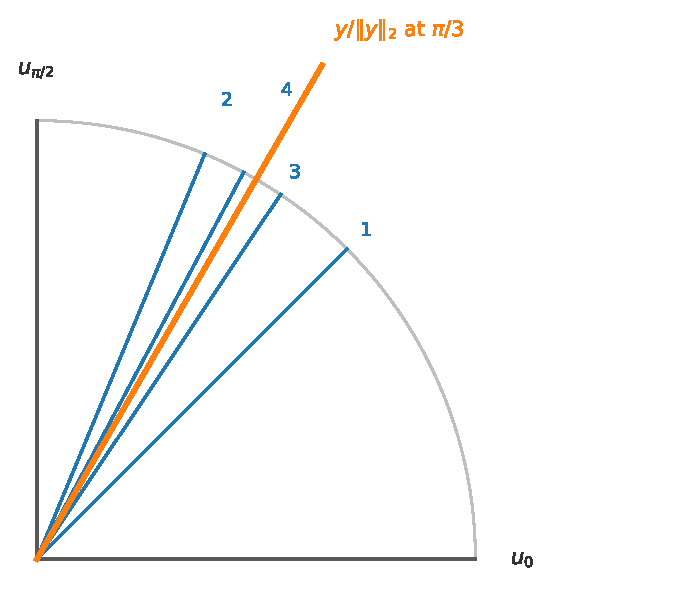
\includegraphics[width=0.45\linewidth]{figures/bisection_construction.pdf}
  \caption{The nontermination instance of Theorem~\ref{t-nontermination}.
  From the atoms $u_0,u_{\pi/2}$, exact pricing adds the angular midpoint of
  the bracketing pair in every round (first four additions numbered). The
  target direction at angle $\pi/3$ is approached by bisection and never
  reached.}
  \label{f-bisection}
\end{figure}

\section{The complexity of pricing}\label{s-pricing}

The analysis so far confines the difficulty to the pricing oracle. This
section maps its complexity: pricing
is a Boolean quadratic problem in disguise, which makes it NP-hard in
general---but the same structure makes it boundable (\S\ref{s-bounds}),
tractable at fixed effective rank, and coverable by sampling when the target
chambers are wide.

As a computational problem: given rational $X$, $\nu$, and rational $c$,
\emph{pricing} asks whether $p(\nu)\ge c$; the approximation version asks for
a direction whose price is at least a constant fraction of $p(\nu)$.

\begin{lemma}[Positive-part Boolean collapse]\label{l-boolean}
For $w\in\reals^n$ with $w\ge0$ entrywise, with $\odot$ the componentwise
product,
\[
  \rho(w)=\max_{s\in\{0,1\}^n}\norm{X^T(s\odot w)}_2 .
\]
\end{lemma}

\begin{proof}
For fixed $u$, maximizing $\sum_i s_iw_ix_i^Tu$ over $s\in\{0,1\}^n$ selects
exactly the positive entries of $Xu$ and recovers $w^T\relu{Xu}$; the finite
maximum over $s$ commutes with the maximum over the unit ball, and
$\max_{\norm u_2\le1}(s\odot w)^TXu=\norm{X^T(s\odot w)}_2$.
\end{proof}

\begin{theorem}[Pricing is hard]\label{t-hardness}
Pricing is NP-hard and APX-hard on rational inputs, already for $\nu=\ones$.
Consequently it admits no polynomial-time approximation scheme unless
$\mathrm P=\mathrm{NP}$. The reduction does not exclude a fixed-constant
approximation.
\end{theorem}

\begin{proof}
Let $A_G\in\{-1,0,1\}^{|E|\times|V|}$ be an oriented incidence matrix of an
unweighted graph $G$ and set $X=A_G^T$, so $n=|V|$ and $d=|E|$. For
$s\in\{0,1\}^{|V|}$, the vector $A_Gs$ has one entry per edge, equal to $\pm1$
exactly on edges cut by $s$; hence by Lemma~\ref{l-boolean},
\[
  \rho(\ones)^2=\max_{s\in\{0,1\}^{|V|}}\norm{A_Gs}_2^2
  =\operatorname{MaxCut}(G).
\]
Since $\rho(\ones)^2$ is an integer, a rational $c$ with $c^2\in(k-1,k]$,
computable in polynomial time, makes the question $p(\ones)\ge c$ decide
$\operatorname{MaxCut}(G)\ge k$; the gap instances likewise admit rational
thresholds.
ReLU features are nonnegative, so $\rho(-\ones)=0$ and
$p(\ones)=\rho(\ones)$. The construction is rational. A direction whose price
is within a factor $1/(1+\delta)$ of optimal induces, through its positive
gate, a cut within $1/(1+\delta)^2$ of the maximum cut, so Max-Cut gap
hardness \citep[Theorem~8.2]{hastad2001optimal} gives NP-hardness,
APX-hardness, and the no-PTAS consequence. Conversely, a cut containing at
least half the edges always exists and yields a direction with price at least
$\rho(\ones)/\sqrt2$, so the squared transfer cannot rule out every fixed
constant.
\end{proof}

The hard instances have $d=|E|$ growing with the graph; hardness is a
large-rank phenomenon. At fixed effective rank the whole problem---not just
pricing---is tractable to prescribed accuracy.

\begin{theorem}[Fixed effective rank]\label{t-fixed-rank}
Suppose $X,y,\lambda$ are rationally encoded, $\lambda>0$, and $r=\rank X$ is
fixed. Enumerating all full-dimensional chamber closures gives a rational
second-order cone program (SOCP) of size polynomial in the input. For
rational $\epsilon>0$, one can compute in time polynomial in the input length
and $\log(1/\epsilon)$ a point violating each conic constraint by at most
$\epsilon$ whose objective is within $\epsilon$ of optimal, in the standard
weak conic model.
\end{theorem}

\begin{proof}
Proposition~\ref{p-chamber-count} bounds the number of closures polynomially
for fixed $r$, and arrangements in fixed dimension are enumerable in
polynomial time \citep{edelsbrunner1986constructing}. The sign inequalities,
norm epigraphs, and a rotated-cone epigraph for the squared loss form a
rational SOCP \citep[\S4.4.2]{boyd2004convex}; the zero point bounds the total
block mass by $\norm y_2^2/(2\lambda)$, so the relevant level set is bounded,
and weak conic optimization gives the stated accuracy
\citep[Chapters~4 and~6]{nesterov1994interior}.
\end{proof}

This is full enumeration at prescribed accuracy; it neither returns exact
irrational optima in the bit model nor bounds the number of RCG rounds.

The remaining positive result concerns the cheapest oracle of all: random
directions. Selected-pattern solvers \citep{mishkin2022fast,kim2024sampling}
rely on sampled gates, and multistart search needs seeds; both are governed by
how much of the sphere the relevant chambers occupy. For a gate $s$ let $C_s$
denote its chamber and $\mu(s)=\Pr\{g\in C_s\}$ its Gaussian measure, with
$g\sim\mathcal N(0,I_r)$ in the row span. Say a finite set $T$ of chambers is
\emph{covered} by sampled directions when each chamber in $T$ contains at
least one of them.

\begin{proposition}[Coverage of a fixed target set]\label{p-coverage}
For $N$ independent Gaussian directions and a finite target set $T$,
\[
 \Pr\{T\text{ is covered}\}\ \ge\ 1-\sum_{s\in T}(1-\mu(s))^N ,
\]
so with $\mu_{\min}=\min_{s\in T}\mu(s)$, a budget
$N\ge\mu_{\min}^{-1}\log(|T|/\delta)$ covers $T$ with probability at least
$1-\delta$. If $r\ge2$ and a chamber $C_s$ contains a center $\bar u$ with
normalized margin
\[
 m_0=\min_{i:\,\norm{x_i}_2>0}
 \frac{|x_i^T\bar u|}{\norm{x_i}_2\norm{\bar u}_2}>0,
\]
then
\begin{equation}\label{e-cap-mass}
 \mu(s)\ge\frac{m_0^{\,r-1}}{\pi(r-1)} .
\end{equation}
\end{proposition}

\begin{proof}
The union bound gives the coverage statement. The angular distance from
$\bar u$ to every nonzero row hyperplane is at least $\arcsin m_0$, so the
open spherical cap of that radius stays inside the chamber; integrating its
surface measure and using concavity of sine gives \eqref{e-cap-mass}. The
case $r=1$ is elementary on the two-point sphere.
\end{proof}

The direction of this result matters. A lower bound on chamber mass gives an
upper bound on a sufficient sampling budget; it cannot prove that a chamber is
small or that exponentially many samples are \emph{necessary}. (If every
nonzero row equals $e_1^T$, the positive chamber has mass $1/2$ in every
dimension.) What sampling actually does to the fitting objective, as measured
margins shrink with dimension, is an empirical question we take up in
\S\ref{s-exp-curse}.

\section{Computable price bounds}\label{s-bounds}

Exact pricing is hard, but a valid \emph{upper bound} on the price is still
useful twice over: it can pass the stopping test $p(\nu)\le\lambda$ when
search cannot, and through the dual \eqref{e-dual} it scales the residual into
a feasible dual point and hence an objective lower bound. This section
constructs such bounds from the Boolean collapse, in exact arithmetic, and
develops a $d\times d$ dual so that no $n\times n$ semidefinite object is ever
formed: the $n$-sized operations are two batched matrix products, and one
evaluation costs $O(nd^2)$.

\subsection{Two bounds from the Boolean collapse}

Fix $\nu$ and put $w=\nu_+=\max(\nu,0)$. Negative residual entries only lower
the one-sided score, so $\rho(\nu)\le\rho(w)$. Define
\[
  b_0=X^Tw,
  \qquad
  \widehat B=\begin{bmatrix}b_0^T\\ \diag(w)X\end{bmatrix}\in
  \reals^{(n+1)\times d},
\]
with rows indexed $0,1,\ldots,n$. Substituting $s=(\ones+\varepsilon)/2$ in
Lemma~\ref{l-boolean} and using the sign symmetry $z\mapsto-z$,
\[
  \rho(w)
  =\frac12\sqrt{\max_{z\in\{-1,1\}^{n+1}}z^T\widehat B\widehat B^Tz}
  \ \le\
  \bar\rho_{\rm joint}(\nu)
  :=\frac12\sqrt{\operatorname{SDP}(\widehat B\widehat B^T)},
\]
where the first equality is exact and
\[
  \operatorname{SDP}(G)
  =\max\{\ip{G}{Y} \mid Y\succeq0,\ \diag(Y)=\ones\}
\]
is the standard semidefinite relaxation of Boolean quadratic maximization.
Nesterov's bound \citep{nesterov1998semidefinite} gives
$\bar\rho_{\rm joint}(\nu)\le\sqrt{\pi/2}\,\rho(\nu_+)$: past the sign
truncation $\rho(\nu)\le\rho(\nu_+)$, the joint form is within the absolute
constant $\sqrt{\pi/2}\approx1.25$ of what it bounds.

A second bound follows from the split $\relu t=(t+|t|)/2$: since
$\nu^T\relu{Xu}\le w^T\relu{Xu}=\tfrac12w^TXu+\tfrac12\sum_iw_i|x_i^Tu|$,
bounding the linear term by Cauchy--Schwarz and relaxing the sign
maximization in the second term by the same SDP gives
\[
 \bar\rho_{\rm split}(\nu)
 =\frac12\norm{X^T\nu_+}_2
  +\frac12\sqrt{\operatorname{SDP}
  \left(\diag(\nu_+)XX^T\diag(\nu_+)\right)} .
\]
The split form discards the coupling between the linear and Boolean parts and
carries no constant-factor comparison; the joint form loses only the sign
truncation beyond the SDP relaxation. Both are valid for their sign, and both
remain valid when $\operatorname{SDP}(\cdot)$ is replaced by any upper bound
on it---which is what the next subsection supplies.

\subsection{A small-cone dual}\label{s-small-cone}

The relaxation $\operatorname{SDP}(BB^T)$ for $B\in\reals^{q\times d}$ has a
$q\times q$ variable, unusable at $q\approx n$. Its diagonal dual is
classical \citep{delorme1993laplacian}; the identity below re-expresses that
dual over the $d\times d$ cone, which we call the \emph{small-cone form}.

\begin{theorem}[Small-cone dual identity]\label{t-small-cone}
Let $B\in\reals^{q\times d}$ have rows $b_i^T$. In exact arithmetic,
\begin{align}
 \operatorname{SDP}(BB^T)
 &=\min_{\eta\in\reals^q}
   \{\ones^T\eta \mid \diag(\eta)\succeq BB^T\}
 \label{e-diag-dual}\\
 &=\max_{Z\succeq0}
   \Big(2\sum_i\sqrt{b_i^TZb_i}-\Tr Z\Big).
 \label{e-small-cone}
\end{align}
Zero rows of $B$ contribute zero terms to the sum in \eqref{e-small-cone} and
may be deleted; after deleting them, every feasible $\eta$ in
\eqref{e-diag-dual} is entrywise positive and the matrix constraint is
equivalent to $B^T\diag(\eta)^{-1}B\preceq I$.
\end{theorem}

\begin{proof}
The primal SDP has the strictly feasible point $Y=I$, so strong duality holds
and the dual minimum in \eqref{e-diag-dual} is attained. Delete zero rows;
congruence and equality of nonzero singular values give the inverse-form
constraint. Dualizing that constraint with multiplier $Z\succeq0$ separates
over coordinates, and for each row
\[
  \inf_{t>0}\Big(t+\frac{b_i^TZb_i}{t}\Big)=2\sqrt{b_i^TZb_i}.
\]
A large positive multiple of $\ones$ is strictly feasible in
\eqref{e-diag-dual}, so the exchange of $\min$ and $\max$ is exact, giving
\eqref{e-small-cone}.
\end{proof}

The right side of \eqref{e-small-cone} is a concave function of the $d\times
d$ variable $Z$, maximized by a few projected gradient steps whose $n$-sized
work is the two batched products $\diag(BZB^T)$ and $B^T\diag(\cdot)B$. The
essential feature is that an \emph{inexact} $Z$ still yields a valid bound:

\begin{proposition}[Recovering a diagonal bound]\label{p-recovery}
Delete zero rows of $B$. Choose any positive weights $\bar c_i>0$ and form
\[
  M=\sum_i\frac{b_ib_i^T}{\bar c_i}.
\]
If $\bar\lambda_M$ is an exact or certified upper bound on
$\lambda_{\max}(M)$, then $\eta_i=\bar\lambda_M\bar c_i$ is feasible in
\eqref{e-diag-dual}, so
\begin{equation}\label{e-recovered}
  \operatorname{SDP}(BB^T)\le\bar\lambda_M\sum_i\bar c_i .
\end{equation}
\end{proposition}

\begin{proof}
With $\eta_i=\bar\lambda_M\bar c_i$, the inverse-form constraint of
Theorem~\ref{t-small-cone} reads $B^T\diag(\eta)^{-1}B=M/\bar\lambda_M\preceq
I$, which holds by the definition of $\bar\lambda_M$.
\end{proof}

In practice one takes $\bar c_i$ near $\sqrt{b_i^TZb_i}$ for an approximately
optimal $Z$, floored away from zero; the floor is sound only if the floored
values are the ones used to form $M$.

\paragraph{From price bounds to a dual bound.}
Evaluate the bounds separately per sign and take, within each sign, the
minimum of the valid forms:
\[
 \bar\rho_+=\min\{\bar\rho_{\rm joint}(\nu),\bar\rho_{\rm split}(\nu)\},\quad
 \bar\rho_-=\min\{\bar\rho_{\rm joint}(-\nu),\bar\rho_{\rm split}(-\nu)\},\quad
 \bar p=\max\{\bar\rho_+,\bar\rho_-\}\ \ge\ p(\nu),
\]
in exact arithmetic, with $\operatorname{SDP}(\cdot)$ replaced throughout by
the recovered bound \eqref{e-recovered}. Maximizing the dual objective
$D$ of \eqref{e-dual} along the ray $\xi=\theta\nu$ over the certified
interval $0\le\theta\le\lambda/\bar p$ gives
\[
 \theta=
 \begin{cases}
  0,&\nu=0,\\
  \max\{\nu^Ty/\norm\nu_2^2,\,0\},&\nu\ne0,\ \bar p=0,\\
  \max\{\min(\nu^Ty/\norm\nu_2^2,\ \lambda/\bar p),\,0\},
      &\nu\ne0,\ \bar p>0,
 \end{cases}
\]
and $D(\theta\nu)$ is then a lower bound on $J^\star$. A valid price bound
thus becomes a computable optimality gap for any feasible model.

\begin{remark}[Floating-point status]\label{r-floating}
Equations \eqref{e-diag-dual}--\eqref{e-recovered} are exact algebra. Our
implementation accumulates $M$ in round-to-nearest floating point and calls a
standard symmetric eigensolver, and that computed value can lie \emph{below}
the exact $\lambda_{\max}(M)$: with scalar rows $b_1=1$, $b_2=2^{-27}$ and
$\bar c_1=\bar c_2=1$, the exact value $1+2^{-54}$ rounds to $1$, and taking
$\bar\lambda_M=1$ makes $\diag(\eta)-BB^T$ indefinite. Inflating the final
scalar by one unit in the last place would cover this example but not errors
accumulated earlier in the products and the eigensolve. A rigorous bound
requires \emph{outward} (directed) evaluation---each floating operation
rounded in the direction that provably preserves the inequality, as in
interval arithmetic---applied to the accumulation of $M$, the spectral bound,
and the evaluation of the primal and dual objectives, and it should fail
closed: report failure rather than an unverified bound. Until that path
exists, the gap fields our solver reports are numerical estimates, and we
flag them as such wherever they appear.
\end{remark}

\subsection{What semidefinite rounding does and does not give}
\label{s-rounding}

The same relaxation, rounded, proposes directions. Let
$B=\diag(|\nu|)X$, let $G=BB^T$, and define the symmetrized objective
$h(u)=\sum_i|\nu_i||x_i^Tu|$ with maximum $h^\star$ over the unit ball.
Suppose $Y\succeq0$, $\diag(Y)=\ones$, and $\ip{G}{Y}\ge\kappa
\operatorname{SDP}(G)$ for a proved $0<\kappa\le1$. Choose Gram vectors $v_i$
with $Y_{ij}=v_i^Tv_j$, draw a standard Gaussian $g$, set
$\varepsilon_i=\mathop{\bf sign}(v_i^Tg)$, and let
$u_\varepsilon=B^T\varepsilon/\norm{B^T\varepsilon}_2$ (zero if
$B^T\varepsilon=0$).

\begin{proposition}[Symmetrized rounding]\label{p-rounding}
Assume $h^\star>0$ and let $a_\kappa=2\kappa/\pi$. Then
$\mathbf{E}\,h(u_\varepsilon)^2\ge a_\kappa\,(h^\star)^2$, and for every
$0\le\zeta<a_\kappa$, one draw satisfies
\[
 \Pr\{h(u_\varepsilon)\ge\sqrt\zeta\,h^\star\}
 \ge\frac{a_\kappa-\zeta}{1-\zeta}.
\]
For an exact SDP optimizer ($\kappa=1$), the choice $\zeta=1/\pi$ gives
factor $1/\sqrt\pi$ with probability at least $1/(\pi-1)$; independent draws
amplify this threshold.
\end{proposition}

\begin{proof}
The hyperplane-rounding identity gives
$\mathbf{E}\,\varepsilon^TG\varepsilon\ge(2/\pi)\ip{G}{Y}$
\citep{goemans1995improved}, and pointwise
$h(u_\varepsilon)\ge\norm{B^T\varepsilon}_2$, so
$\mathbf{E}\,h(u_\varepsilon)^2\ge(2/\pi)\ip{G}{Y}\ge a_\kappa(h^\star)^2$,
using $(h^\star)^2=\max_\varepsilon\varepsilon^TG\varepsilon\le\operatorname{SDP}(G)$.
Normalizing by $(h^\star)^2$ yields a variable $Q\in[0,1]$ with
$\mathbf{E}\,Q\ge a_\kappa$; if $q_0=\Pr\{Q\ge\zeta\}$ then
$a_\kappa\le\zeta(1-q_0)+q_0$, the tail bound.
\end{proof}

This proposition controls $h$, not mixed-sign ReLU pricing, and the gap
between the two can be arbitrarily large. With rows $e_1,e_1,e_2$ and residual $(L,-L,1)$,
every exact SDP optimizer has $Y_{12}=1$, so rounding gives
$\varepsilon_1=\varepsilon_2$ almost surely; then
$B^T\varepsilon=(\pm2L,\pm1)$, and even checking both orientations, the best
ReLU price obtained is $1/\sqrt{4L^2+1}$ while $p(\nu)=1$: the ratio tends to
zero. There is no uniform conversion from symmetrized to signed pricing. Our
solver therefore uses rounding only to \emph{propose} directions and always
evaluates their actual ReLU scores.

\paragraph{Observed tightness.}
Two exploratory observations (floating point, single runs) locate these
bounds in practice. On ten small
random instances where the price could be computed exactly by enumeration,
the joint small-cone estimate exceeded the exact price by factors
$1.4$--$2.5$, where an earlier additive variant of the bound (using $|\nu|$ in
place of $\nu_+$) read $2.3$--$7.4$,
and every evaluation was numerically valid against the enumerated truth. On
adversarial Max-Cut pricing instances ($|V|=8$--$16$, eight graphs per size),
hyperplane-rounded proposals recovered the enumeration-exact optimum in every
trial (ratio $1.000$), while gradient ascent from random starts, with the activation mask held fixed
within each step as in \S\ref{s-production}, averaged $0.974$--$0.995$ of it.

\section{The RCG solver}\label{s-production}

The implemented solver keeps the objective and gives up the exact premises.
Heuristics generate candidate directions; a candidate is accepted only when
the full-data objective of problem \eqref{e-finite-atom} accepts it, and every
returned model is feasible for that problem. The ideal method's premises
degrade as follows. The exact master becomes a
floating active-set lasso with a small ridge term, tolerances, and an
iteration cap. Exact pricing becomes a sketched multistart ascent whose
survivors are rescored on all rows. The optional moves of
Proposition~\ref{p-optional} become gated consolidation, pruning, capping,
and orientation-sensitive deduplication, none of which retains the
proposition's premises---so the rate \eqref{e-rate} and the stopping
guarantee of Corollary~\ref{c-restricted-stop} are statements about the ideal
method, not this solver. What survives is feasibility, the unchanged
objective, and an independently recomputed cost for every returned model.
Algorithm~\ref{alg-production} shows one production round; the paragraphs
below define its steps.

\begin{algorithm}[tb]
\caption{Production RCG (one round)}\label{alg-production}
\begin{algorithmic}[1]
\Require data $X,y$; penalty $\lambda$; working set; sketch rows $S$;
  per-sign append budget $n_{\rm add}$ (default $8$); column cap
\State \textbf{master:} solve the atom lasso numerically (warm active set,
  cached Gram columns, ridge, tolerances); gather the residual $\nu$
\State \textbf{consolidate:} solve the gated proposal \eqref{e-gated} on a
  sketch; refit the projected directions on all rows; \textbf{accept only if}
  the full-data cost does not increase
\State \textbf{price:} run sketched multistart ascent on $\pm\nu$; rescore
  survivors on all rows; retain orientation-distinct finalists per sign
\State \textbf{add:} append up to $2n_{\rm add}$ violators
  ($|a^T\nu|>\lambda$), deduplicated with orientation; refit; prune tiny
  coefficients; compress same-chamber groups; cap the working set
\State \textbf{diagnose:} update the price-based and bound-based gap
  estimates; stop on any rule in the stopping paragraph below
\end{algorithmic}
\end{algorithm}

\paragraph{Master.}
Over the working set $\{u_1,\ldots,u_P\}$ the master is the lasso on the
feature matrix $A=[\,a(u_1)\ \cdots\ a(u_P)\,]$, whose columns are the
working set's atoms. Atoms drawn from nearby
directions are highly correlated, which motivates a warm-started primal
active-set method \citep{osborne2000new}: on the active set the KKT system is
a small dense solve, sign-infeasible coordinates are dropped, and the most
violating inactive atom enters, with a small ridge for conditioning and
tolerances and an iteration cap for termination. Gram columns are computed
once, in float64, when an atom first enters; the only $n$-sized master
operation per step is one correlation product $A^T\nu$.

\paragraph{Gated consolidation.}
Adding one atom at a time can stall in a way no single-atom move repairs:
several active atoms straddle a better direction, and re-aiming any one of
them alone increases the cost. The escape move is joint. Freeze each active
atom's activation pattern on a sketch---its \emph{gate}
$s_j=\ones\{X_Su_j\ge0\}$, where $S$ is a uniformly drawn row subset and
$X_S$, $y_S$ denote the corresponding rows of $X$ and $y$, with the penalty
rescaled by $|S|/n$---and solve the group lasso
\begin{equation}\label{e-gated}
\begin{array}{ll}
\mbox{minimize} & \displaystyle
    \frac12\norm{\sum_{j=1}^P s_j\odot(X_Sz_j)-y_S}_2^2
    +\frac{|S|}{n}\,\lambda\sum_{j=1}^P\norm{z_j}_2,
\end{array}
\end{equation}
with variables the blocks $z_1,\ldots,z_P$, by block coordinate descent. The
minimizer transports mass between atoms, deletes redundant blocks through
group sparsity, and re-aims the survivors jointly. Because the gates are
frozen, \eqref{e-gated} is \emph{not} the fitting objective; it is only a
proposal. Each nonzero block is normalized to a direction, the true ReLU
atoms are rebuilt, and the refit on all rows replaces the working set only if
the computed full-data cost does not increase. We call this whole step
\emph{gated consolidation}; its cost appears as a named phase in
\S\ref{s-experiments}.

\paragraph{Pricing search.}
Production pricing is a sketched multistart ascent. Its sketch is an
importance sample: rows are drawn with probability proportional to
$|\nu_i|\norm{x_i}_2$ and reweighted so the sketched correlation is an
unbiased estimate of $\nu^T\relu{Xu}$. Seeds combine the normalized residual
correlation $X^T\nu$, leading singular directions of $\diag(\nu)X$ (spectral
seeds), the active atoms and perturbations of them, surviving directions from
previous rounds, and random draws. From each seed, projected gradient ascent
maximizes the sketched estimate over the unit ball with the activation mask
frozen within each step; writing $g$ for the mask-frozen sketch gradient and
$\omega>0$ for a fixed damping coefficient, one iteration either scores both
the normalized gradient and the damped step
$(u+\omega g)/\norm{u+\omega g}_2$ (the \emph{two-trial} update) or only the
damped step (the \emph{damped} variant). Both residual signs are searched
together. The highest-scoring orientation-distinct survivors per sign---the
\emph{finalists}, where $u$ and $-u$ are never identified (see working-set
maintenance below)---are rescored on all rows, and only full-data scores
decide what is appended.

\paragraph{Candidate ordering.}
Raw signed correlation $|a^T\nu|$ remains the violation test. The exact
one-coordinate decrease of appending an atom against a fixed residual,
\begin{equation}\label{e-decrease}
   \Delta(a)=
   \begin{cases}
    \dfrac{\relu{|a^T\nu|-\lambda}^2}{2\norm a_2^2},&a\ne0,\\[1ex]
    0,&a=0,
   \end{cases}
\end{equation}
can instead rank the candidates that pass it. Ranking is all it does---the
violation quantity is unchanged---and correlation ordering remains the
default because predicted-decrease ordering did not earn its extra cost in
the controlled comparison of \S\ref{s-exp-controlled}.

\paragraph{Working-set maintenance.}
Accepted atoms are refit, tiny coefficients are pruned, and the working set
is capped; capping is applied only after a newly appended atom has
participated in a refit, and pruning is followed by another refit, so the
solver never prices a stale residual. Two operations deserve definitions.
\emph{Orientation-sensitive deduplication:} ReLU is not odd, so $u$ and $-u$
are different atoms---for $X=(1,-1)^T$ the directions $u=1$ and $u=-1$ have
absolute cosine one yet produce the orthogonal features $(1,0)^T$ and
$(0,1)^T$---and deduplication therefore never identifies $u$ with $-u$.
\emph{Chamber compression:} active atoms sharing a chamber and sign are
merged by the conic combination $v=\sum_{j\in\mathcal G}|\alpha_j|u_j$, which
leaves the prediction unchanged and can only decrease the penalty
($\norm v_2\le\sum_{j\in\mathcal G}|\alpha_j|$ since all $u_j\in K_s$); this is an
exact improvement, applied when eligible groups appear.

\paragraph{Precision.}
Feature-side quantities (atom builds, screening, candidate rescoring) involve
no cancellation and run in float32, where accelerators deliver their
throughput. The master's KKT correlations $a_j^T\nu$ cancel catastrophically
as the residual shrinks, so the master, the residual accumulation, and the
small spectral factorizations run in float64. Returned objectives are
recomputed in float64.

\paragraph{Sharding.}
The engine row-shards $X$ and the residual across CPU blocks or
CUDA/ROCm devices. Atom construction leaves full-height features on their
shards; screening, Gram construction, rescoring, spectral seeds, and bound
evaluation end in host reductions whose sizes depend on $P$, the candidate
count, or $d$---not on $n$. The design is shard-ready rather than
communication-optimal: each round still gathers an $O(n)$ residual to the
host, and chamber handling can move $O(nP)$ masks, so communication grows
with the sample count. Physical multi-CPU and multi-GPU speedups have not
been measured; \S\ref{s-exp-controlled} reports the one placement experiment
we have.

\paragraph{Stopping and reported diagnostics.}
The solver stops when any of the following holds: the price-based gap
estimate falls below a relative threshold; the search finds no violator (after
one retry with escalated search budgets); the objective decrease over a patience window of six
rounds is below $10^{-7}$ relative while the best found price is within $5\%$
of $\lambda$ (plateau); every finalist deduplicates against the working set
(no new distinct column); or a time budget or round cap is reached.
Tolerance-based stopping is forced, not chosen: Theorem~\ref{t-nontermination}
shows even exact RCG need not terminate. The returned model always carries an
independently recomputed full-data objective, a valid upper bound on
$J^\star$. Two gap estimates accompany it: a \emph{bound-based gap estimate}, the
floating evaluation of the bound-and-dual construction of \S\ref{s-bounds}
(an estimate for the reasons of Remark~\ref{r-floating}), and a
\emph{price-based gap estimate} that substitutes the best found price---a
lower bound on $p(\nu)$---where a valid upper bound belongs, and can
therefore understate the true gap. Neither
certifies optimality, and the solver labels both accordingly.

\paragraph{Defaults.}
Unless stated otherwise the experiments use the solver's fixed defaults---no
per-instance tuning: at most $100$ rounds, up to $16$ appended atoms per
round across the two signs, a working-set cap of $512$ columns, gated
consolidation every round with at most $100$ block passes, and sketches of
$32{,}768$ rows once $n$ exceeds $65{,}536$ (full data below that): an
importance sample for pricing, and a uniform subsample for gated
consolidation that grows up to $4\times$ after rejected proposals.

\section{Numerical experiments}\label{s-experiments}

Our evidence comes in two grades, and we label every result with its grade.
\emph{Controlled} experiments follow a preregistered protocol: one or two
warm-up runs, three or more measured repeats per variant in balanced order (a
cyclic Latin schedule, so each variant occupies each position within one
count), synchronized accelerator timing, process-level page-fault and swap
checks, and \emph{objective replay}---the returned $(U,\alpha)$ re-evaluated
on the full data by an independent code path. Variants are compared at
matched quality: a candidate's replayed objective must be within
$10^{-4}\max\{1,|F_{\rm baseline}|\}$ of the baseline's (the \emph{quality
envelope}). Because these comparisons set the solver's defaults, decision
rules were fixed before measuring: a variant replaces the default only on a
$20\%$ median end-to-end reduction, and a placement change must not regress
runtime by more than $10\%$. \emph{Exploratory} results are single
unreplicated runs, with objectives computed by the solver or driver as
described and wall-clock measured in an unrecorded machine power state; we
use them for orders of magnitude and cross-method comparisons of objective
values, not for fine timing claims. The accompanying result records include
the configurations, raw measurements, and run metadata. The hardware
throughout is one laptop: an AMD Ryzen~7~7735U (eight cores, sixteen
threads, OpenBLAS and OpenMP capped at eight threads) with an integrated
Radeon~680M GPU reached through Torch/ROCm.

\subsection{Planted instances (exploratory)}\label{s-exp-planted}

We first ask whether the solver reaches good objective values at all, on
instances where a strong reference value is available. A \emph{planted}
instance draws $X$ with i.i.d.\ standard normal entries and sets $y$ as the
noiseless output of $k$ fixed teacher atoms; the \emph{teacher reference} is
the lasso solved over the teacher's own atoms, a feasible upper bound on
$J^\star$ (not a proven optimum).

Across five planted configurations spanning $n=500$ to $5000$, $d=12$ to
$32$, and $k=3$ to $8$, the solver's returned objective exceeded the teacher
reference by between $6\times10^{-6}$ and $9.6\times10^{-5}$ relative, in
$0.3$ to $9.3$ seconds, with the search still pricing about $4\%$ above
$\lambda$ at exit. For calibration, a single-column refinement baseline
(per-atom refinement, no gated consolidation)
finished $2\%$ to $56\%$ above the reference on four of the five instances
(it was not run on the fifth) while taking $5$--$15\times$ longer---the gap that motivated the gated step. On one
instance small enough to enumerate all $818$ patterns ($n=30$, $d=3$), the
heuristic search returned the enumeration-exact price in all ten rounds, and
the final exact price exceeded $\lambda$ by less than $10^{-8}$: consistent
with global optimality up to master tolerances, on that instance only.

Against tuned baselines, on a planted $n=10^5$, $d=16$, $k=3$ instance: RCG
reached objective $0.31408$ (test MSE $1.3\times10^{-10}$, seven active
atoms) in $42$ seconds; Adam, AdamW, and SGD---width $64$, each grid point of
three learning rates $\times$ two seeds given the \emph{full} $42$-second
budget, roughly six times RCG's total compute per optimizer---ended at best
objectives of $2018$, $1672$, and $1966$ respectively (best test MSE
$0.035$), with grid medians $4$--$10\times$ their bests. On this
teacher-realizable instance the first-order methods do not approach the
convex optimum at any grid point.

\subsection{Sampling and dimension (exploratory)}\label{s-exp-curse}

A natural question is whether residual-guided pricing offers a real advantage
over random sampling of patterns. Proposition~\ref{p-coverage} says sampling
covers wide chambers cheaply; the empirical question is what happens to the
fitting objective as the relevant chambers narrow. On planted instances with
$n=50$, $k=2$, and $d$ from $2$ to $16$ (three repeats each), the measured
minimum teacher-chamber solid angle falls from $1.3\times10^{-2}$ at $d=2$ to
below the $5\times10^{-6}$ Monte Carlo resolution by $d=8$
(Figure~\ref{f-curse}a). At a fixed budget of $40$ chambers, both selection
rules use the same exact lasso master and differ only in where the chambers
come from: random Gaussian gates versus residual-guided search. Sampling's
objective degrades by up to $2.4\times$ as $d$ grows while the
residual-guided objective stays flat (Figure~\ref{f-curse}b). This is the
practical face of the collapse theorem: priced atoms are placed by the
residual, and random ones rarely land in the active chambers once those are
narrow. These runs used the reference chamber implementation; the comparison
isolates column \emph{selection}. A direct comparison with selected-pattern
solvers would confound selection with master implementations and stopping rules, so we
leave it to the next-steps list in \S\ref{s-conclusion}.

\begin{figure}[tb]
  \centering
  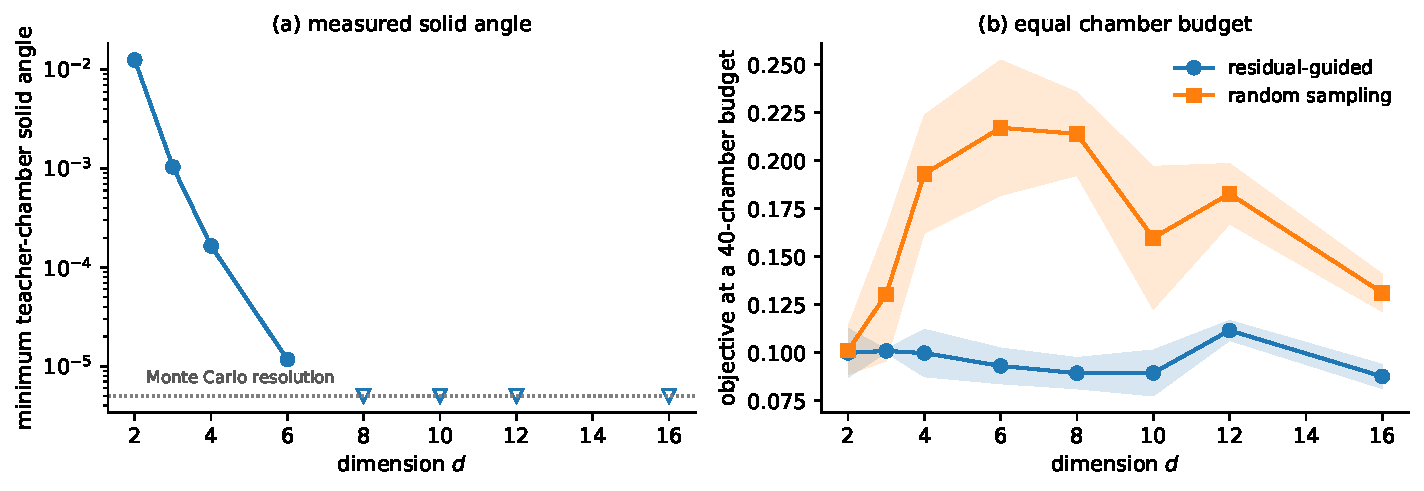
\includegraphics[width=\linewidth]{figures/dimension_sampling.pdf}
  \caption{Sampling and dimension, planted $n=50$, $k=2$ (exploratory; means
  and standard deviations over three repeats). (a)~Measured minimum
  teacher-chamber solid angle; open markers indicate values below the Monte
  Carlo resolution of $5\times10^{-6}$. (b)~Objective at a fixed
  $40$-chamber budget: random gates versus residual-guided selection through
  the same exact master.}
  \label{f-curse}
\end{figure}

\subsection{Real data (exploratory)}\label{s-exp-realdata}

We now compare the solver with tuned first-order baselines on real data at
budget-matched wall clock. Three datasets: California housing ($15{,}480\times9$
after split), Covtype ($435{,}759\times55$, least-squares classification of
one class), and YearPredictionMSD ($386{,}509\times91$). Protocol: a $75/25$
train/test split (seed $0$), features and target standardized by training
statistics, bias column appended; $\lambda$ set to $10^{-2}$ times a sketch
estimate of the smallest $\lambda$ with empty solution; every method
minimizes the same objective, with baselines scored on the weight-decay form
\eqref{e-weight-decay} recomputed from their final weights in float64.
RCG ran with a $30$-round cap, its one non-default setting for these runs,
and the matched budget $T$ below is its wall clock under that cap. Baselines
are width-$128$ networks, minibatched at large $n$. The tuning grids are
budget-matched to $T$: Adam (three learning rates
$\times$ three seeds) and SGD (five learning rates $\times$ three seeds)
each receive $T$ in total, split evenly per run; AdamW's decoupled decay
rate needs its own sweep (five values at Adam's per-run budget), so its grid
total is $1.67\,T$. On California the grid totals are floored at $20$ seconds against $T=17$,
an overshoot that favors the baselines. Divergent runs (non-finite
objectives) are dropped from best and median statistics; SGD kept $12/15$,
$6/15$, and $6/15$ runs on the three datasets. Three further asymmetries, disclosed: an unbalanced network's
weight-decay cost exceeds the atomic cost of the same predictor, so baseline
objectives can be slightly overstated (exact per-neuron rebalancing would
remove this, but the saved records contain objectives, not weights); RCG's objective is the solver's final
full-data float64 value rather than the controlled protocol's independent
replay; and Adam's best learning rate landed at the grid edge on California
and MSD, so those grids may not bracket its optimum.

\begin{table}[tb]
\centering
\footnotesize
\setlength{\tabcolsep}{4pt}
\resizebox{\linewidth}{!}{%
\begin{tabular}{llrrrrr}
\toprule
Dataset & Method & Objective & vs.\ RCG & Test MSE & Runs & Time \\
\midrule
California & RCG (32 atoms) & $2457$ & --- & $0.263$ & 1 & $17$ s\\
$n=15{,}480$, $d=9$ & Adam best / median & $4445$ / $8433$ & $+81\%$ / $+243\%$
  & $0.273$ & 9 & $20$ s total\\
& AdamW best / median & $4936$ / $7845$ & $+101\%$ / $+219\%$ & $0.396$ & 15 &
  $33$ s total\\
& SGD best / median & $9628$ / $15337$ & $+292\%$ / $+524\%$ & $0.509$ & 12 &
  $20$ s total\\
\midrule
Covtype & RCG (85 atoms) & $133911$ & --- & $0.563$ & 1 & $1137$ s\\
$n=435{,}759$, $d=55$ & Adam best / median & $126528$ / $129229$ &
  $-5.5\%$ / $-3.5\%$ & $0.512$ & 9 & $1137$ s total\\
& AdamW best / median & $130501$ / $140806$ & $-2.5\%$ / $+5.1\%$ & $0.530$ &
  15 & $1896$ s total\\
& SGD best / median & $152790$ / $236315$ & $+14\%$ / $+76\%$ & $0.562$ & 6 &
  $1137$ s total\\
\midrule
MSD & RCG (101 atoms) & $134741$ & --- & $0.669$ & 1 & $1959$ s\\
$n=386{,}509$, $d=91$ & Adam best / median & $130105$ / $130250$ &
  $-3.4\%$ / $-3.3\%$ & $0.644$ & 9 & $1959$ s total\\
& AdamW best / median & $130963$ / $134208$ & $-2.8\%$ / $-0.4\%$ & $0.647$ &
  15 & $3265$ s total\\
& SGD best / median & $145757$ / $218601$ & $+8.2\%$ / $+62\%$ & $0.669$ & 6 &
  $1959$ s total\\
\bottomrule
\end{tabular}%
}
\caption{Real data at budget-matched wall clock (exploratory; single runs). All
methods minimize the same objective; ``vs.\ RCG'' is the signed relative
difference of the method's objective from RCG's. Test MSE is in
target-variance units, best run shown for baselines. ``Total'' times are
tuning-grid totals; see the protocol text for per-run budgets and the AdamW
exception.}
\label{tab-realdata}
\end{table}

Table~\ref{tab-realdata} and Figure~\ref{f-realdata} give the results. The
outcome splits by dataset. On California, RCG's objective is $45\%$ below
the best tuned grid point ($81\%$ of RCG's value above it), the tuned medians
are $3.2$--$6.3\times$ RCG's value, and held-out MSE follows the same order; the
solver's price-based gap estimate fell below $1\%$ of the objective at
round $24$. On Covtype and MSD, RCG stopped at its $30$-round cap with the
search still pricing atoms at $1.7$--$2.0\times\lambda$---columns remained
to add---and the best tuned Adam runs finished $5.5\%$ and $3.4\%$ lower,
with correspondingly lower test MSE. Two observations temper the losses.
The tuned methods pay a tuning bill the convex method does not: SGD's median
run is $50$--$55\%$ above its own best on the large datasets, and it
diverges outright at learning rates large enough to move fast ($9$ of $15$
runs on each large dataset). And RCG's exits are round-capped, not
converged, so its large-dataset values are not the method's limit. We do not
attribute the split to a property of the optima (such as sparsity); with the
tools of this paper that would be conjecture, and we leave it as one.

\begin{figure}[tb]
  \centering
  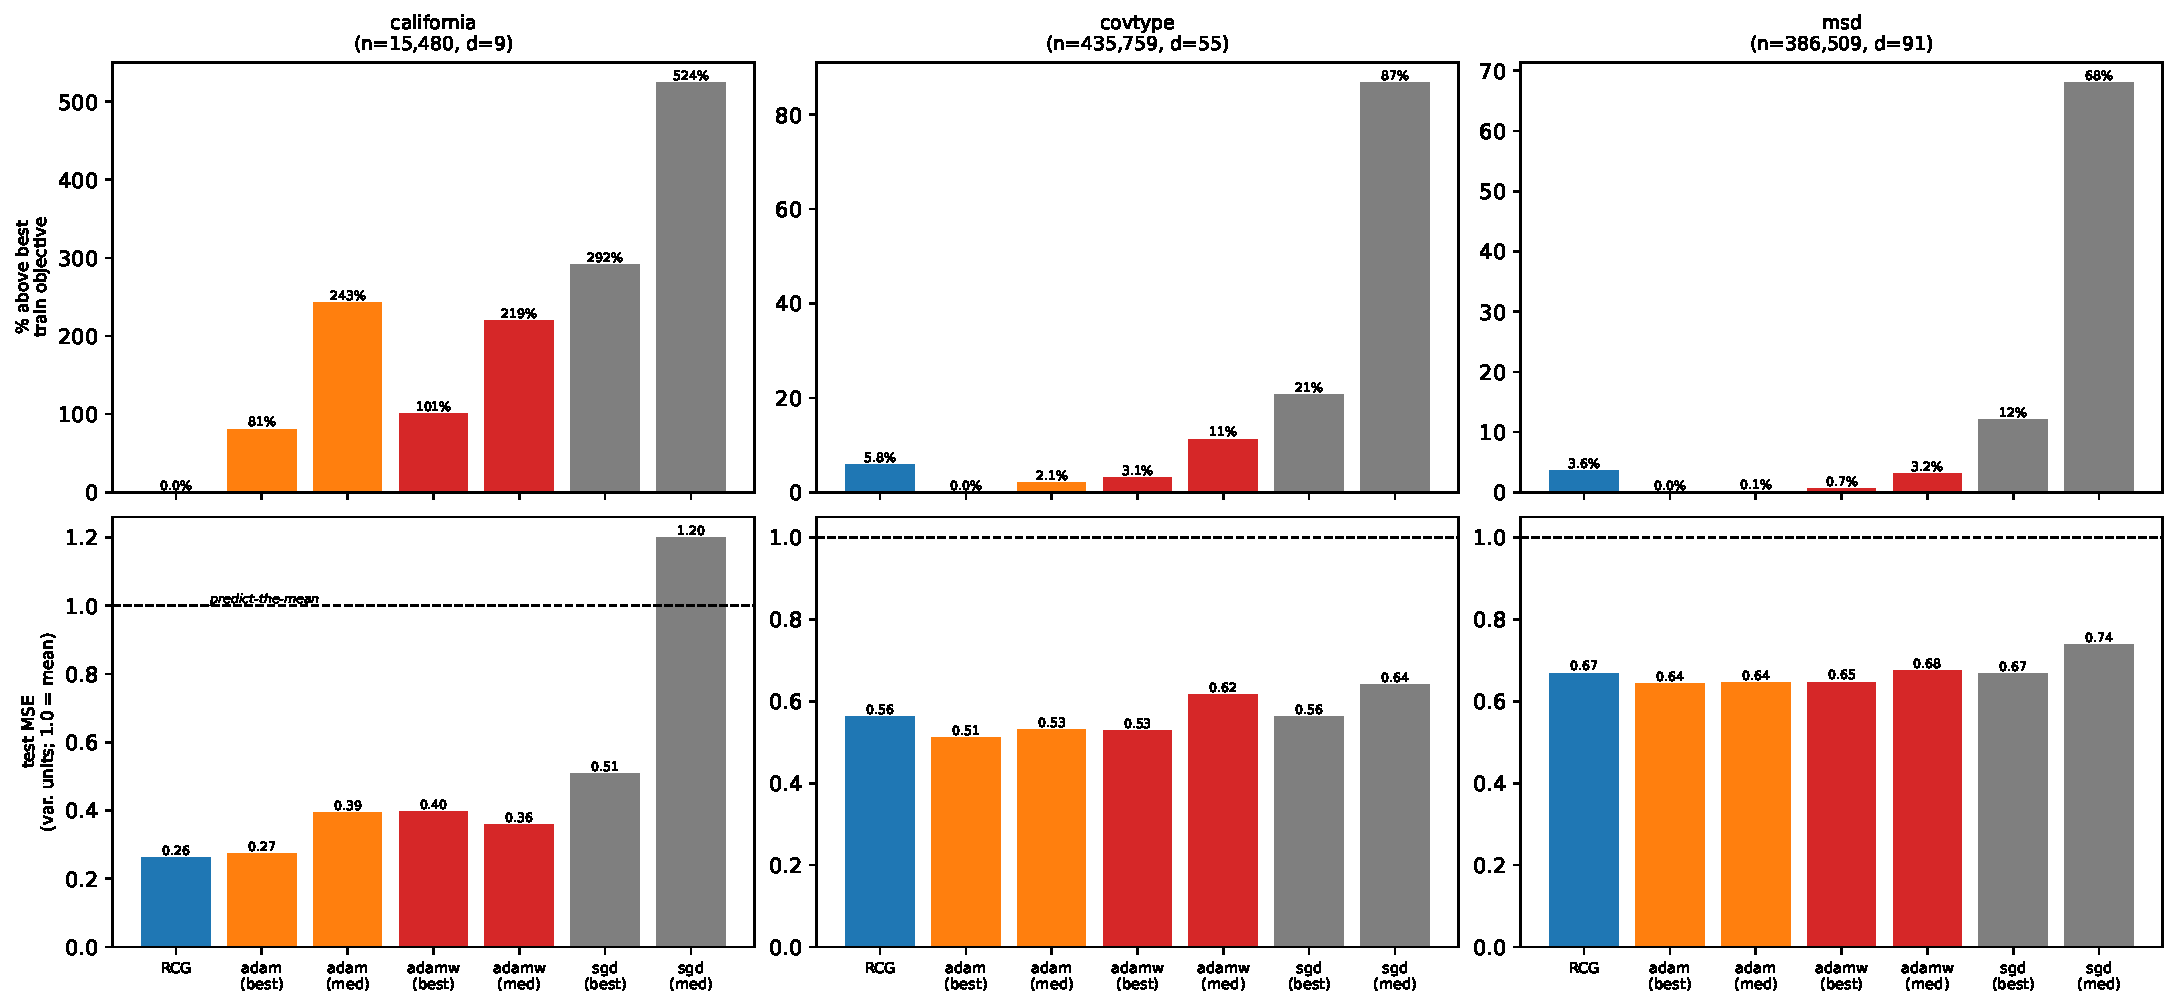
\includegraphics[width=\linewidth]{figures/real_data_comparison.pdf}
  \caption{Real-data comparison at matched wall clock (exploratory). Top:
  training objective as percent above the per-dataset best. Bottom: held-out
  MSE in target-variance units; the dashed line is predict-the-mean.}
  \label{f-realdata}
\end{figure}

\subsection{Scale (exploratory)}\label{s-exp-scale}

On planted instances at fixed $d=16$, $k=3$, single CPU runs under a
$60$-round cap: $n=2\times10^4$ ran in $24.8$ seconds, $10^5$ in $50$ seconds, $5\times10^5$ in $75$
seconds, and $2\times10^6$ in $173$ seconds---$100\times$ the rows for
$7\times$ the time---with returned objectives between $+3.9\times10^{-5}$ and
$+1.3\times10^{-3}$ relative to the teacher reference (itself only a feasible
upper bound). These are not convergence claims: every run at $n\ge10^5$
reached the round cap with the search still reporting violations,
increasingly so at scale (up to $6.4\times\lambda$ at $n=2\times10^6$). The
sublinear growth reflects sketch-bounded search plus $O(n)$ full-data
passes, consistent with the communication accounting of
\S\ref{s-production}. At $n=10^6$ a paired run of the same Torch engine put
the integrated GPU at $115$ seconds versus $109$ on the CPU---an early hint,
confirmed under protocol below, that accelerator residency is not
automatically a win on this shared-memory machine.

\subsection{Controlled implementation experiments}\label{s-exp-controlled}

The controlled experiments ask configuration questions about the solver
itself, under the protocol and decision rules stated at the top of this
section. The end-to-end instance is a deterministic planted problem with
$n=10^4$, $d=16$, three teacher atoms, $\lambda=0.1$, seed zero.

\paragraph{CPU variants.}
Three single-host NumPy configurations: the default (two-trial ascent,
correlation ordering), damped ascent alone, and damped ascent with
predicted-decrease ordering. Table~\ref{tab-cpu} reports medians of three
measured runs after one warm-up; all replayed objectives pass the quality
envelope. Damped ascent alone removes one forward product per search
iteration yet is $2.5\%$ slower end to end; combined with predicted-decrease
ordering it is $18.2\%$ faster---short of the $20\%$ bar, so the default
stands. No measured process incurred a major page fault or acquired swap,
though system-wide swap activity was recorded as an interference warning
during some runs. The phase decomposition (Figure~\ref{f-phases}) is the real
finding: the combined variant cuts pricing search from $2.69$ to $1.22$
seconds, at which point gated consolidation ($2.89$ s) becomes the largest
phase; further pricing reductions would now have limited effect on the total,
and the gated phase is the natural next target.

\begin{table}[tb]
\centering
\small
\begin{tabular}{lrrrr}
\toprule
Variant & Objective & Time (s) & IQR (s) & Ratio \\
\midrule
two-trial, correlation (default) & 0.3209115 & 5.447 & 0.069 & 1.000 \\
damped, correlation & 0.3209134 & 5.581 & 0.497 & 1.025 \\
damped, predicted-decrease & 0.3209221 & 4.456 & 0.187 & 0.818 \\
\bottomrule
\end{tabular}
\caption{CPU variants at $n=10^4$, $d=16$ (controlled). Medians over three
balanced-order measured runs after one warm-up; IQR is the interquartile
range of the three runs by linear-interpolation quartiles, and Ratio is
median time over the default's. All objectives are independently replayed
and pass the quality envelope.}
\label{tab-cpu}
\end{table}

\begin{figure}[tb]
  \centering
  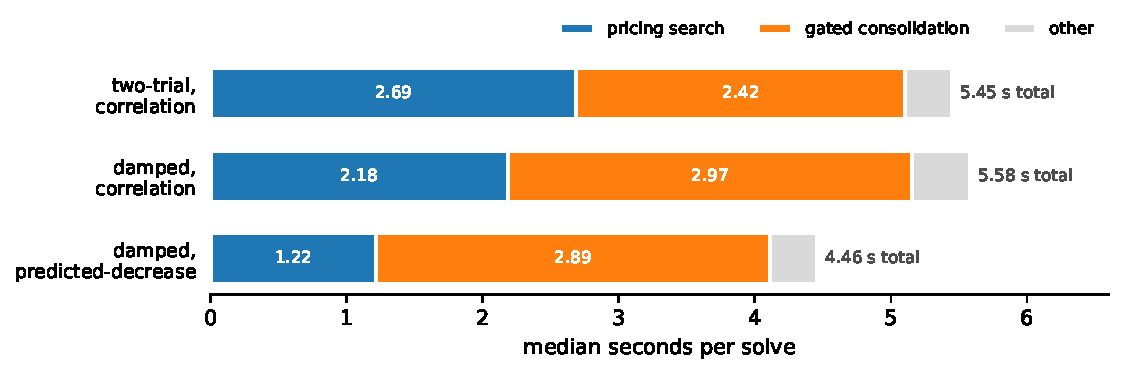
\includegraphics[width=0.9\linewidth]{figures/runtime_breakdown.pdf}
  \caption{Where the time goes: per-phase median seconds for the three CPU
  variants of Table~\ref{tab-cpu}. Cutting pricing search exposes gated
  consolidation as the dominant phase.}
  \label{f-phases}
\end{figure}

\paragraph{Candidate-ordering and reuse probes.}
A probe that replays one component in isolation tested candidate ordering
across $20$ saved solver states ($960$ scalar checks of the identity
\eqref{e-decrease} against directly computed one-coordinate updates---all
passed). Predicted-decrease ordering changed the selection in only $3$ of
$20$ states; on those reversals its
median fully-refit gain was $0.59\times$ correlation's, and computing the
candidate norms it needs made rescoring $1.65\times$ slower. A second probe
tested reusing the finalists' already-built feature columns instead of
rebuilding them: at $n=1.2\times10^5$, $d=64$ (eight balanced repeats after
two warm-ups), reuse reproduced the same eight oriented directions and
features exactly but took $1.07\times$ the rebuild path's time, with a
$38$~MB peak memory increase against a $\approx1.8$~GB ceiling. Both
alternatives remain available as non-default options.

\paragraph{Device placement.}
Holding the Torch float32 engine fixed and moving only the pricing search to
the integrated GPU: host search took a median $7.67$ seconds (IQR $0.09$),
device search $11.07$ seconds (IQR $1.72$)---$44\%$ slower, failing the
$10\%$ regression rule, with the entire loss in the pricing phase ($6.13$
versus $2.30$ seconds). The result concerns one shared-memory integrated GPU
and says nothing about discrete or multiple GPUs; host search remains the
local default.

\section{Conclusions}\label{s-conclusion}

Convexity moves the hardness of two-layer ReLU fitting into a separation
oracle, and this paper analyzed that oracle in both directions. With an exact
oracle, column generation carries full optimality conditions and an $O(1/t)$
rate that never sees the exponential chamber count---but provably need not
terminate, so tolerance-based stopping is intrinsic to the problem, not a
concession of the implementation. Without one, pricing is NP-hard and
APX-hard already at the all-ones residual, yet boundable: a $d\times d$
semidefinite dual upper-bounds the price in exact arithmetic and converts any
valid bound into an objective gap. In between sits the implemented solver,
which accepts a heuristic proposal only when the full-data objective does,
preserving feasibility and the objective while giving up the exact
premises, and whose measured behavior is competitive: near-reference values
on planted data, robustness to dimension at a fixed working-set budget where
random
sampling degrades, a $45\%$ objective win over tuned baselines on one real
dataset and $3.4$--$5.5\%$ losses on two others at budget-matched wall clock, and a
phase profile that names gated consolidation as the next bottleneck.

The limitations are equally concrete. The comparative evidence is
exploratory: single runs, solver-computed objectives, unrecorded machine
power state; the controlled protocol currently covers only implementation
variants on one planted instance and one machine, with three repeats. The
floating bound path is not outward-evaluated, so the solver reports gap
estimates, not certificates. And the real-data losses occurred at round caps,
so the convex method's large-scale limit is unmeasured. The corresponding
next steps are mechanical to state: extend the round caps on the two losing
datasets, where the search was still finding violators; rerun the real-data
comparison under the controlled protocol, with baselines scored on rebalanced
weights; compare directly against selected-pattern solvers such as SCNN and
CRONOS at matched budgets; implement the outward (directed) bound evaluation
of Remark~\ref{r-floating}, fail-closed, which is one directed-rounding
engineering pass; attack the gated phase; and measure discrete-GPU and
multi-device execution on hardware that has it.

One mathematical question stands out. In exact arithmetic, the only
structural slack in the positive-part route of \S\ref{s-bounds} is the sign
truncation $\rho(\nu)\le\rho(\nu_+)$: closing it requires a relaxation that
couples the gate pattern of a direction with the direction itself, and we
know of no published bound that exploits this realizability structure. We
leave it as the main open problem.

\paragraph{Code and result availability.}
The implementation, result records, and complete reproduction instructions
are available in the \href{https://github.com/epicycloids/relu-chambers}{online
supplement}. The controlled records include raw measurements, data and model
digests, and software and hardware metadata; the exploratory records preserve
their configurations, seeds, tuning grids, and budgets.

\appendix

\section{The nontermination construction}\label{a-nontermination}

We prove Theorem~\ref{t-nontermination}. Let $X=I_2$, $\lambda=1$, and
$y=4u_{\pi/3}$, where $u_\theta=(\cos\theta,\sin\theta)$, and initialize the
master with the atoms of $u_0=e_1$ and $u_{\pi/2}=e_2$. In the positive
quadrant the price of a nonnegative residual is its Euclidean norm. By the
projection characterization of the restricted dual (\S\ref{s-optimality}),
the exact restricted dual solution is the Euclidean projection of $y$ onto
$\{\nu \mid |u_\theta^T\nu|\le1\text{ for every accumulated }\theta\}$; along
the constructed trajectory the lower inequalities are inactive. Initially
the projection is $(1,1)$, so exact pricing adds $u_{\pi/4}$.

Suppose adjacent accumulated angles $\varphi_1<\pi/3<\varphi_2$ bracket the
target. Write $\varphi_m=(\varphi_1+\varphi_2)/2$ for the midpoint and
$h=(\varphi_2-\varphi_1)/2$ for the half-width. The two tangent lines meet at
$v=\sec(h)\,u_{\varphi_m}$. The projection normal-cone condition at $v$
reduces to
\[
  4\sin(2h/3)\ \ge\ \tan h,
\]
which holds for $0<h\le\pi/4$ by the elementary chord bounds for sine and
tangent; and $v$ satisfies every non-adjacent accumulated constraint because
$\sec(h)\cos(\theta-\varphi_m)\le1$ whenever $|\theta-\varphi_m|\ge h$. Thus
$v$ is the exact restricted dual solution, and exact pricing adds the
midpoint angle $\varphi_m$.

The target $\pi/3$ sits at relative position $2/3$ of $[0,\pi/2]$ and remains
at relative position $1/3$ or $2/3$ of the bracketing interval after every
bisection; it is never a dyadic midpoint. Hence every finite round has price
$\norm v_2=\sec h>1=\lambda$ and adds a new atom. The bracket shrinks, so
$J_t\to J^\star$, but the algorithm never stops. \qed

\small
\bibliographystyle{abbrvnat}
\bibliography{references}

\end{document}
